\section{Funciones}

\subsection{Funciones, gráficas y relaciones}

Supongamos que para cada elemento de un conjunto $A,$ asignamos un \emph{único} elemento de un conjunto $B;$ diremos que la colección de tales asignaciones es una \emph{función} de $A$ en $B.$ 


En tal caso, denotamos escribimos 
$$f:A\to B, \; a \mapsto f(a)$$
donde $f(a)\in B$ es la asignación correspondiente a $a\in A.$



La conexión entre \emph{funciones} y \emph{relaciones} es la siguiente:


Definimos la gráfica de una función $f:A\to B$ como el subconjunto de $A \times B$
$$
\Gamma_{f}=\set{(a, f(a)) \mid a \in A}.
$$


 $f:A\to B$ es una función si su gráfica es una relación tal que $$(a,b), (a,b')\in \Gamma_{f} \onlyif b=b'.$$  
\emph{Observe que $\Gamma_{f}$ es una relación en $A\times B.$}

En este caso, diremos que $a\in A$ es la \emph{varible independiente,} mientras que $b\in B$ es la \emph{variable dependiente.}



De manera reciproca, una relación $R\subset A \times B$ induce una función si 
$$
(a,b), (a,b')\in R \onlyif b=b'.
$$


En tal caso (abusando de la notación), la función está definida por 
$$
R:A\to B, \; a \mapsto b:=R(a).
$$



Entonces, una relación no induce una función si...


El conjunto $A$ es llamado \emph{dominio} de la función, y al conjunto $B$ se le conoce \emph{codominio.}


La \emph{imagen} de una función $f:A\to B$ se define como
\begin{align*}
	\imagen{f}&={\color{red} f(A)}\\
	&=\set{b \in B \mid \exists a \in A: b=f(a)}\\
	&=\set{f(a)\in B \mid a \in A}
\end{align*}

Frecuentemente, una función puede expresarse por medio de una fórmula matemática. 
\begin{ejemplo}
	Consideremos la función que asigna a cada número real su cuadrado. Podemos describir esta función escribiendo
	$$
	f(x)=x^{2} \texttt{ o } x\mapsto x^{2} \texttt{ o } y=x^{2}.
	$$
\end{ejemplo}



En el ejemplo anterior, la gráfica de $f:\R \to \R$ esta dada por 
$$
\Gamma_{f}=\set{(x,y)\in \R^{2}\mid y=x^{2}}
$$ y es una parábola.


Mientras que la imagen de $f$ esta dada por 
$$
f(\R)=\set{x^{2}\mid x\in \R}=\set{y\in \R \mid y\geq 0}.
$$



\begin{ejemplo}
	La relación 
	$$
	R=\set{(x,y)\in \R^{2}\mid x^{2}+y^{2}=1}
	$$
	no induce una función.
\end{ejemplo}




\begin{ejemplo}
	Sea $A$ un conjunto arbitrario. La función $:A \to A$ que asigna a cada elemento $a\in A$ el mismo elemento es llamada \emph{identidad,} usualmente denotada por $\id_{A}$ o simplemente $\id$
	
	
	En otras palabras, la identidad está definida por $$
	\id:A\to A, \; a \mapsto \id(a)=a.
	$$ Observe que
	$$
	\Gamma_{\id_{A}}=\triangle_{A}.
	$$
\end{ejemplo}



 
 \begin{ejemplo}
  Supongamos que $S \subset A.$ La \emph{inclusión} de $S$ en $A,$ denotada por $i: S \hookrightarrow A$ esta dada por $i(x)=x.$
 
 
 Observe que es la asignación es similar a la identidad, pero el dominio está restringido a $S \subset A.$
 
 
 La \emph{restricción} $f\mid_{S}$ de una función $f:A \to B$ a $S \subset A$ esta dada por
 $$
 f\mid_{S}: S \to B, \; x\mapsto f(x).
 $$
 \end{ejemplo}
 
 

\subsection{Composición de Funciones}


Consideremos dos funciones $f:A \to B$ y $g:B \to C.$ Podemeos definir una nueva función $:A \to C$ de la siguiente manera
$$
a \mapsto {\color{purple}b=f(a)} \mapsto c=g({\color{purple}b})=g({\color{purple}f(a)}).
$$


La función anterior se conoce como \emph{composición} $g$ con se $f$ se describe de la siguiente manera
$$
\begin{cases} 
	{\color{red} g\circ f}:A\to C \\ 
	x \mapsto {\color{purple}g(f(x))}.
\end{cases}
$$




\subsection{Funciones inyectivas, suprayectivas e inversas}


\begin{definicion} Consideremos una función $f:A\to B.$ Diremos que
	\begin{enumerate}
		\item $f$ es \emph{inyectiva} o \emph{1:1} si $\displaystyle f(a)=f(a')\onlyif a=a'.$ 
		
		\item $f$ es \emph{suprayectiva} o \emph{sobre} si
		$\displaystyle f(A)=B.$ 
		
		\item $f$ es \emph{biyectiva} o \emph{invertible} si la relación inversa de la gráfica $\Gamma_{f}$ induce una función. 
	\end{enumerate}
	
\end{definicion}



\begin{proposicion}
	La función $f:A\to B$ es invertible si y solo si es $1:1$ y sobre.  
	
	En tal caso la relación inversa $R^{-1}$ de $R=\Gamma_{f}$ induce una función denotada por $\displaystyle f^{-1}:B\to A$ tal que
	$$
	\begin{cases}
		f^{-1} \circ f = \id_{A}\\
		f \circ f^{-1} = \id_{B}
	\end{cases}
	$$
\end{proposicion}






\subsection{Como encontrar funciones inversas}


Si $f:A \to B$ no es \emph{sobre,} es decir, $f(A) \subset B$ pero $f(A)\neq B,$ basta restringir su codominio a la imagen $f(A)$ para que se convierta en {sobre}:
$$
f: A \to f(A).
$$



\begin{ejemplo}
	La función $f:\R \to \R, x \mapsto x^{2}$ no es sobre, pero como 
	$$f(A)=\set{x^2\mid x\in\R}=\set{y\in \R \mid y\geq 0}$$
	la función $f: \R\to \set{y \geq 0}, x \mapsto x^{2}$ sí lo es.
\end{ejemplo}




\begin{figure}[h!]
	\centering
	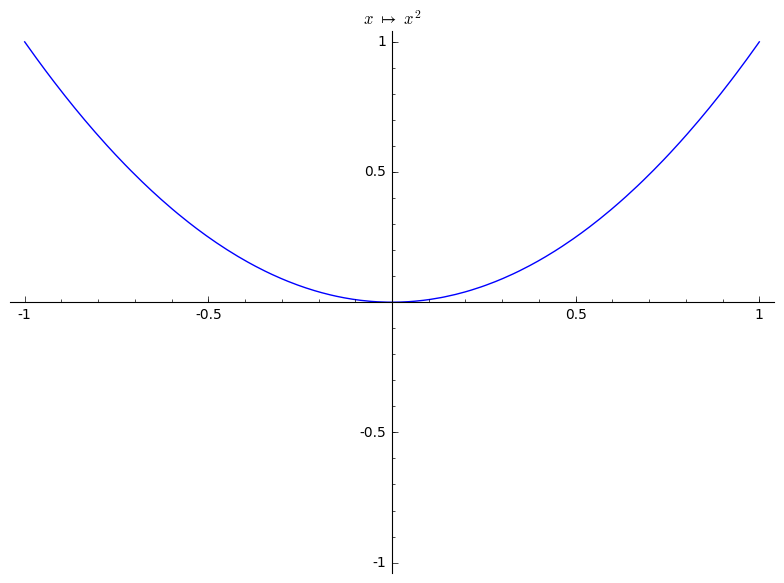
\includegraphics[width=8cm,keepaspectratio=true]{./md/IMG-04_resticcion.png}
	% IMG-04_resticcion.png: 0x0 pixel, 300dpi, 0.00x0.00 cm, bb=
	\caption{Gráfica de $x^2$}
	\label{fig:0401}
\end{figure}




\begin{proposicion}
	Si una función $f:A \to B$ es inyectiva, entonces
	$$
	f:A \to f(A)
	$$ es invertible.
\end{proposicion}



Entonces, para encontrar la inversa de $y=f(x)$, tenemos que:
\begin{enumerate}
	\item Verifique que $f(x)$ es un función $1:1.$ 
	\item Despeje la variable independiente $y$ en la ecuación $y=f(x)$ para obtener
	$$x=f^{-1}(y).$$ 
	\item Reescriba la ecuación anterior intercambiando las variables: $y=f^{-1}(x).$
\end{enumerate}







%
\subsection{Caracterización geom\'etrica}


Considera ahora una función $f:\R \to \R.$ Representemos su gráfica 
$$
\Gamma_{f}=\set{(x,y)\in\R^{2}\mid y=f(x)}
=\set{(x,f(x))}
$$
en el plano.




\begin{observacion}
	\begin{itemize}
		\item $f:\R \to \R$ es \emph{$1:1$} si cada línea \emph{horizontal} intersecta la gráfica de $f$ a lo más en un punto.
		\item $f:\R \to \R$ es \emph{sobre} si cada línea horizontal intersecta la gráfica de $f$ al menos en un punto.
		\item $f:\R \to \R$ es \emph{invertible} si cada línea horizontal intersecta la gráfica de $f$...
	\end{itemize}
	
\end{observacion}




